\graphicspath{{img/ch1}}

\section{Introduction}
Lunar pits are remarkable geological formations that differ significantly from impact craters and volcanic vents. Characterized by steep vertical walls, these features often provide direct access to subsurface voids, such as collapsed lava tubes, tectonic cavities, or impact-induced hollows \cite{lunar-pit-distribution, lunar-pits-entrances-to-caves, new-wagner}. Their discovery, largely enabled by high-resolution imagery from the Lunar Reconnaissance Orbiter (LRO) Narrow Angle Camera (NAC) and the SELENE spacecraft, has revolutionized our understanding of the Moon's crustal architecture, composition, and dynamic history. For example, GRAIL and SELENE data reveal gravity anomalies and radar echoes consistent with intact lava tubes beneath some pits, such as the Marius Hills region \cite{GRAIL, cavities-selene-lavatubes, grails-gradients-mariushills}.

Beyond their geological intrigue, lunar pits hold practical importance for future exploration. These natural formations offer stable thermal environments, shielding from cosmic radiation, and protection from micrometeoroid impacts, making them attractive candidates for human habitation, resource storage, and scientific research stations \cite{bases-feng, newer-thermal, radar-observations-lava-tubes}. Notably, the Mare Tranquillitatis pit (see Fig.~\ref{fig:image1}), a vertical shaft with visible stratigraphic layers, exemplifies the potential of such features to provide insights into lunar geology and serve as access points to extensive cave systems. Radar imaging has further confirmed a subsurface cave conduit beneath the Mare Tranquillitatis pit, supporting its suitability as a target for human exploration \cite{Carrer2024, grails-gradients-mariushills}.

Lunar pits expose ancient stratigraphic layers, revealing records of volcanic flows and crustal evolution. Observations from missions such as SELENE and LRO confirm that these features likely formed through roof collapses above voids, such as lava tubes, highlighting their volcanic origin. For example, the Mare Tranquillitatis pit has been modeled to result from impacts triggering collapses in lava tube roofs, a process corroborated by gravitational anomalies and radar data \cite{lunar-pits-numerical-modelling, radar-observations-lava-tubes, cavities-selene-lavatubes}. The internal layering visible in pits, such as those in Mare Tranquillitatis and Marius Hills, provides key data on successive volcanic episodes, supporting broader studies on lunar surface evolution \cite{sublunear-lava, newer-thermal, bases-feng}.

\begin{figure}[h!]
    \centering
    \begin{subfigure}[c]{0.59\linewidth}
        \centering
        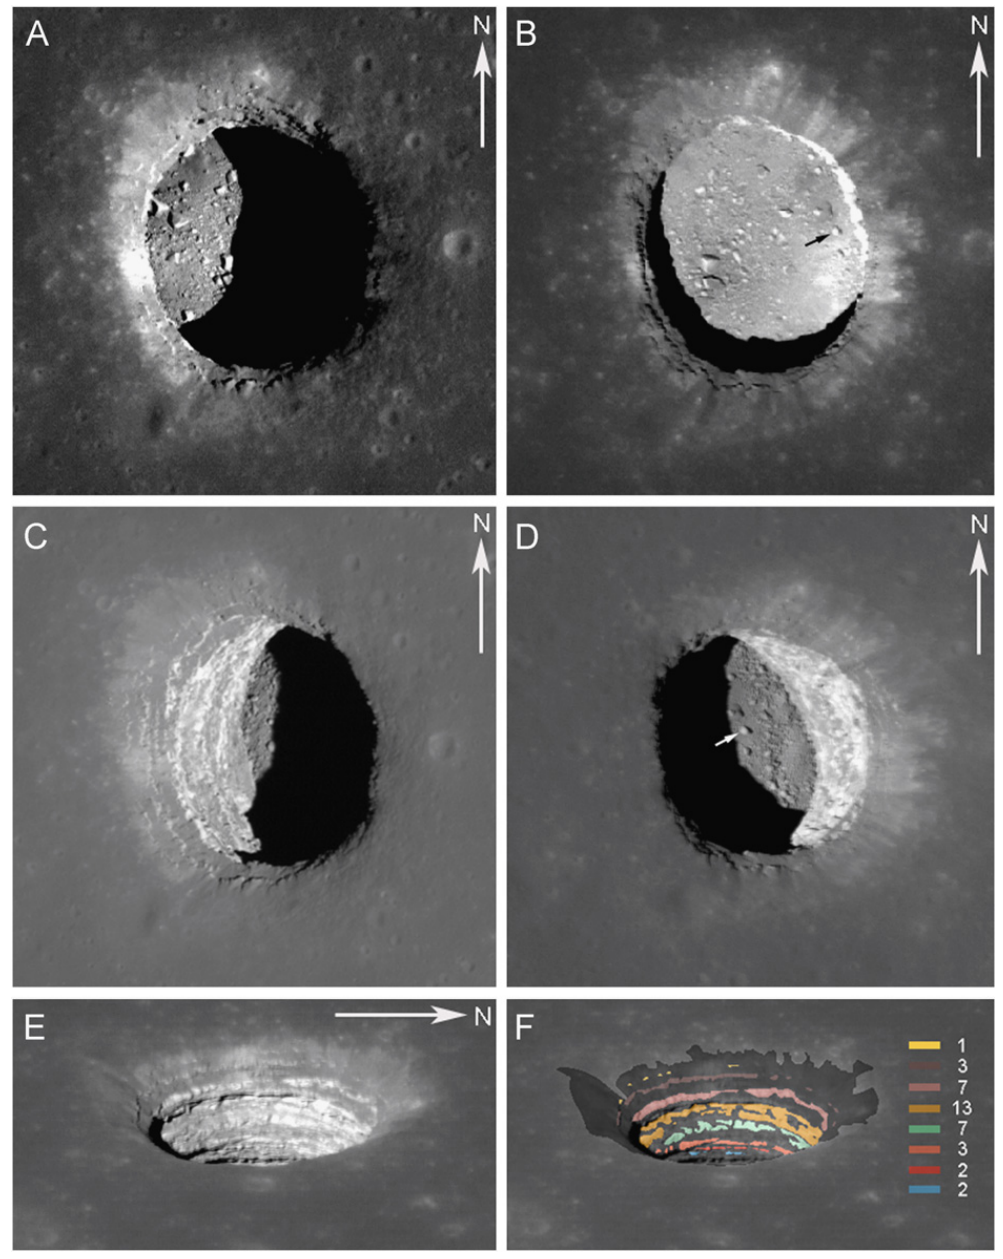
\includegraphics[width=0.9\linewidth]{lunar-pits-with-layers.png}
        \caption{Close-up images of the Mare Tranquillitatis pit, showcasing visible stratigraphic layers (segmentation in Figure \textbf{F}). Images A and B reveal over 90\% of the pit floor using \textbf{LRO NAC} data. Figure adapted from \cite{sublunear-lava}.}
        \label{fig:image1}
    \end{subfigure}
    \hfill
    \begin{subfigure}[c]{0.4\linewidth}
        \centering
        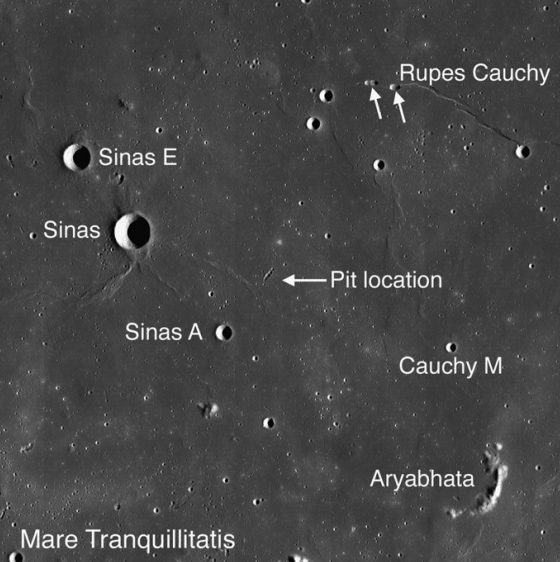
\includegraphics[width=0.9\linewidth]{Lunar_Pit_layers_2pic_location.png}
        \caption{Location of the Mare Tranquillitatis pit, captured by \textbf{LRO WAC}. Figure adapted from \cite{sublunear-lava}.}
        \label{fig:image2}
    \end{subfigure}
\end{figure}

\subsection{Discovery and Recognition}
The identification of lunar pits was delayed until the advent of advanced lunar missions, as these features are relatively small and difficult to observe using Earth-based telescopes \cite{lunar-pit-distribution}. Early evidence emerged from SELENE and LRO data, which revealed steep-walled pits with distinct overhangs and evidence of hollow subsurface structures. For instance, the Mare Tranquillitatis pit has been confirmed to connect to a subsurface void, tens of meters long, using radar and gravitational techniques, transforming pits from geological curiosities to priority targets for lunar exploration \cite{Carrer2024, GRAIL, radar-observations-lava-tubes}.

The Mare Tranquillitatis pit, in particular, has been the focus of radar and imaging studies that confirmed its connection to a subsurface cave conduit. These findings not only demonstrate the scientific value of pits for studying lunar geology but also highlight their potential for human exploration. Advanced thermal modeling, such as that performed using Diviner data, shows that the interior of pits remains thermally stable compared to the extreme surface environment, reinforcing their suitability as habitats or resource storage sites \cite{newer-thermal, lunar-pits-entrances-to-caves, thermal-lunar-pits}.

As technology advances, the exploration of lunar pits continues to evolve. With 3D thermal models, radar imaging, and gravitational studies, these features are increasingly seen as critical to understanding the Moon’s history and unlocking future possibilities for sustained human presence on its surface \cite{newer-thermal, radar-observations-lava-tubes, grails-gradients-mariushills}.